\chapter{Technologies}
\label{chap:Tech}

This chapter covers the different frameworks and technologies that were used to
create Diamond. While many of these technologies provide a wide array of
features, only the features used during the development of Diamond will be
mentioned here. For more in-depth information it is suggested to have a look
at the different documentations.

\section{Angular}

Angular is one of the most popular design frameworks for web applications.
Angular applications are structured in such a way that each visible part of the
app has its own .css, .html and .ts file and is called a component. As with 
other web applications the typescript file contains the logic, the HTML file 
contains the markup and the CSS file defines the look and feel of the component.
TreeTest was originally written in Angular 7 and was updated to the newest 
version of Angular (Angular 11) before development of Diamond began.

\section{Node.js}

Node.js is a JavaScript runtime environment that was used to set up the server 
side of application. It simplifies many of the different web protocol 
interactions and allows developers to handle requests and responses 
asynchronously without having to implement multi threading themselves. Node.js 
was also used to store and retrieve the information stored on the MongoDB 
database.

Additionally, npm is a package manager that comes with Node.js by default, and 
was used to clone all used packages and keep them up-to-date during 
development. This makes the use of external libraries significantly easier and 
reduces the overhead when committing changes to git.

\section{MongoDB}

To store all user related information a MongoDB database was set up. The 
communication between our server and the database was handled by Node.js. 
Furthermore, MongoDB compass was used to visualize the database and manually 
interact with it, in case some erroneous information was stored. A screenshot 
can be seen in Figure~\ref{fig:mongodb_compass}. 


\begin{figure}[tp]  \centering
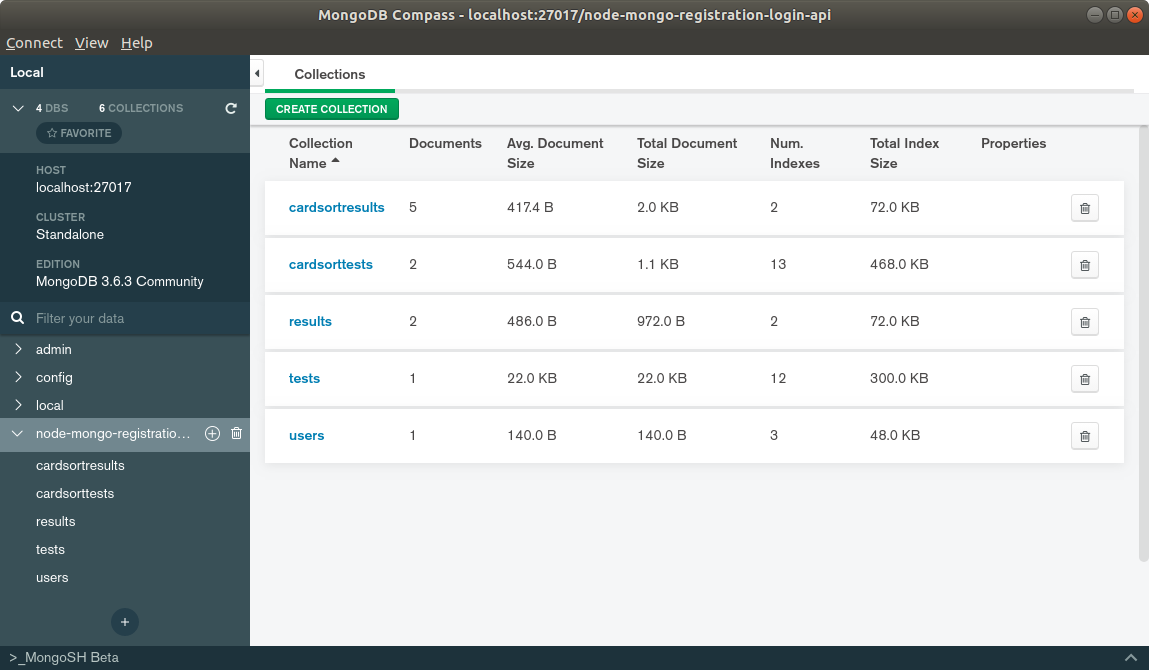
\includegraphics[keepaspectratio,width=\linewidth,height=\halfh]{images/technologies/mongodb_compass.png}
\caption[MongoDB Compass] 
{MongoDB Compass showing the database with some stored information
\imgcredit{Screenshot was captured by Markus Ruplitsch using
MongoDB Compass.} } 
\label{fig:mongodb_compass} 
\end{figure}

\section{Heroku}

Heroku was used for online hosting. In general it is a container-based 
cloud Platform as a Service (PaaS). This means that everything about 
setting up a server, online deployment and hosting is provided by it. It 
is very intuitive to use and free of charge, but an account is needed. 

Heroku offers to connect a GitHub repository to that account. This is 
quite convenient, because you can choose a branch to enable 
auto-deployment after every single push on this branch. For this reason 
you can keep your web application up-to-date very easily. 

It is recommended to created an Heroku branch and to push on that 
branch, when there is a larger number of changes to deploy online. 
And the main branch should just be configured with the localhost 
settings for testing locally.

